\documentclass[tikz,border=5pt]{standalone}
\usetikzlibrary{shapes,arrows.meta,positioning,fit}
\tikzset{
  blk/.style={rectangle,rounded corners,draw=black,fill=blue!8,minimum width=3.4cm,minimum height=0.9cm,align=center},
  mod/.style={rectangle,draw=black,fill=white,minimum width=2.4cm,minimum height=0.8cm,align=center},
  arrow/.style={-{Latex[length=3mm,width=2mm]},thick},
  title/.style={font=\bfseries}
}

\begin{document}
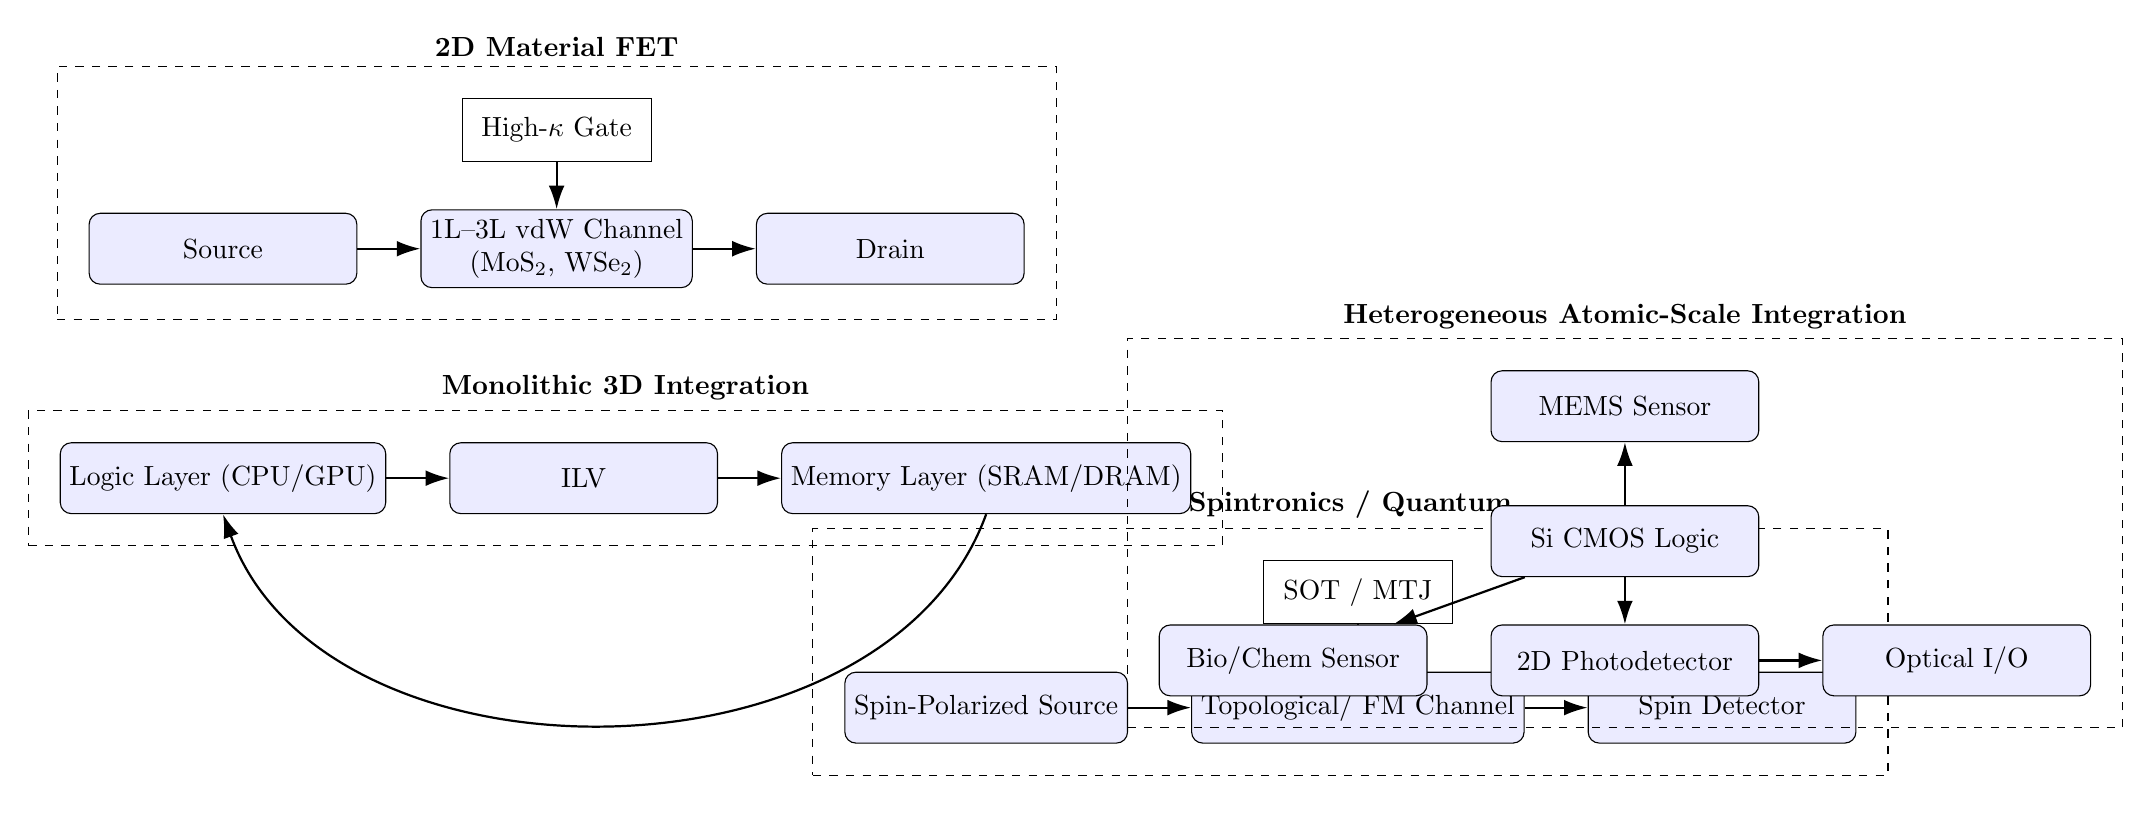
\begin{tikzpicture}[node distance=6mm and 8mm]

% -------- 2D FET --------
\node[blk] (src) {Source};
\node[blk, right=of src] (chan) {1L--3L vdW Channel\\ (MoS$_2$, WSe$_2$)};
\node[blk, right=of chan] (drn) {Drain};
\node[mod, above=6mm of chan] (gate) {High-$\kappa$ Gate};
\draw[arrow] (src) -- (chan);
\draw[arrow] (chan) -- (drn);
\draw[arrow] (gate) -- (chan);
\node[draw=black, dashed, inner sep=4mm, fit=(src)(chan)(drn)(gate), label={[title]above:2D Material FET}] (g2d) {};

% -------- M3D --------
\node[blk, below=20mm of src, xshift=0mm] (logic) {Logic Layer (CPU/GPU)};
\node[blk, right=of logic] (ilv) {ILV};
\node[blk, right=of ilv] (mem) {Memory Layer (SRAM/DRAM)};
\draw[arrow] (logic) -- (ilv);
\draw[arrow] (ilv) -- (mem);
\draw[arrow] (mem.south) to[out=-110,in=-70] (logic.south);
\node[draw=black, dashed, inner sep=4mm, fit=(logic)(ilv)(mem), label={[title]above:Monolithic 3D Integration}] (gm3d) {};

% -------- Spintronics --------
\node[blk, below=20mm of mem, xshift=0mm] (spin_src) {Spin-Polarized Source};
\node[blk, right=of spin_src] (spin_ch) {Topological/ FM Channel};
\node[blk, right=of spin_ch] (spin_det) {Spin Detector};
\node[mod, above=6mm of spin_ch] (sot) {SOT / MTJ};
\draw[arrow] (spin_src) -- (spin_ch);
\draw[arrow] (spin_ch) -- (spin_det);
\draw[arrow] (sot) -- (spin_ch);
\node[draw=black, dashed, inner sep=4mm, fit=(spin_src)(spin_ch)(spin_det)(sot), label={[title]above:Spintronics / Quantum}] (gspin) {};

% -------- Hetero Integration --------
\node[blk, right=38mm of mem, yshift=-8mm] (cmos) {Si CMOS Logic};
\node[blk, below=of cmos] (pd) {2D Photodetector};
\node[blk, right=of pd] (optio) {Optical I/O};
\node[blk, above=of cmos, yshift=2mm] (mems) {MEMS Sensor};
\node[blk, left=of pd] (bio) {Bio/Chem Sensor};
\draw[arrow] (cmos) -- (pd);
\draw[arrow] (pd) -- (optio);
\draw[arrow] (cmos) -- (mems);
\draw[arrow] (cmos) -- (bio);
\node[draw=black, dashed, inner sep=4mm, fit=(cmos)(pd)(optio)(mems)(bio), label={[title]above:Heterogeneous Atomic-Scale Integration}] (ghet) {};

\end{tikzpicture}
\end{document}